\chapter{复变函数与级数}
\rightline{\it 学习复变函数之前要大喊三声:变变变!}
\section{用级数定义一些函数}
什么是复数应该不用我说了。但是你能说清楚$2$的$\rmi$次方是什么意思吗?如果说$\rmi$个$2$相乘就很难理解。现在重新定义一下以前学过的函数,让它们在复数范围内也能用,这些工作叫作\emph{解析延拓}。

前面用级数定义了$\exp x=\sum_{n=0}^{\infty}\frac{1}{n!}x^n=1+x+\frac{1}{2}x^2+\frac{1}{6}x^3+\dots$。不管$x$是实数还是复数,这样的定义都能用。

借助欧拉公式$\exp \rmi x=\cos x+\rmi \sin x$就能定义$\sin x$和$\cos x$。把$\exp \rmi x$打开得到$1+\rmi x-\frac{1}{2}x^2-\frac{1}{6} \rmi x^3+\frac{1}{24} x^4+\frac{1}{120} \rmi x^5-\dots$,然后把实部和虚部分开,得到
\begin{align*}
\sin x&=\sum_{n=0}^{\infty}\frac{1}{(2n+1)!}x^{2n+1}=x-\frac{1}{6}x^3+\frac{1}{120}x^5+\dots \\
\cos x&=\sum_{n=0}^{\infty}\frac{1}{(2n)!}x^{2n}=1-\frac{1}{2}x^2+\frac{1}{24}x^4+\dots
\end{align*}

可以看出$\sin x$是奇函数,$\cos x$是偶函数。为了产生波浪的形状,它们的各项系数是一正一负的。直接求导会发现$\ddx \sin x=\cos x$,$\ddx \cos x=-\sin x$。有兴趣的同学经过一通暴算还会发现$\sin^2 x+\cos^2 x=1$。

但是用级数定义三角函数也有不方便的地方,比如一眼看不出来$\sin \pi=0$(这件事情的证明要等到傅立叶级数),所以有时候我们也会用到几何定义。如果$x$是复数,$\sin x$和$\cos x$的几何意义比较难理解,现在我们只要知道它们是级数就行了。

然后可以定义$\ln x$:如果$\exp x=y$,那么$\ln y=x$。但是奇怪的事情出现了:我们已经知道$\exp 2 \pi \rmi=1$,那么$\ln \exp 2 \pi \rmi=\ln 1$,$2 \pi \rmi=0$?

事实上,不同的$x$可以有相同的$\exp x$,所以$\exp x$的反函数不是单值的,跟反三角函数会出现的问题一样。多值函数的事情以后再讲,现在可以定义:如果$\opIm x \in [0,2\pi)$ 且$\exp x=y$,那么$\ln y=x$。($\opIm x$表示$x$的虚部)

现在任何非零复数的对数都有定义,然后可以定义一般的幂运算:$(a+b \rmi)^{c+d \rmi}=(\rme^{\ln(a+b \rmi)})^{c+d \rmi}=\exp((c+d \rmi)\ln(a+b \rmi))$(要求$a+b \rmi \neq 0$)。这样一来,任何非零复数的复数次方都有了定义,然而零仍然是一个麻烦的问题。

还要注意一下,前面讲的求导和积分都是在一维的情况下的,现在自变量可以在二维的复平面上移动,求导和积分的几何意义都有一些变化,但是之前的公式仍然可以套上去。
\section{三角函数的指数形式;双曲函数}
$\sin x$和$\cos x$可以用$\exp x$表示出来:
\begin{align*}
\sin x&=\frac{1}{2 \rmi}(\rme^{\rmi x}-\rme^{-\rmi x}) & \cos x&=\frac{1}{2}(\rme^{\rmi x}+\rme^{-\rmi x})
\end{align*}

虽然公式中出现了复数,但最后的结果一定是实数。如果把$\rmi$去掉,可以定义:
\begin{align*}
\sinh x&=\frac{1}{2}(\rme^x-\rme^{-x}) & \cosh x&=\frac{1}{2}(\rme^x+\rme^{-x})
\end{align*}

它们叫作双曲正弦和双曲余弦函数,多出来的h表示双曲(hyperbolic)。这就是传说中高中老师不讲,大学老师以为讲过的东西。容易证明以下的关系:(你应该可以口算)
\begin{align*}
\sinh x&=-\rmi \sin \rmi x & \cosh x&=\cos \rmi x \\
\sin x&=-\rmi \sinh \rmi x & \cos x&=\cosh \rmi x \\
\ddx \sinh x&=\cosh x & \ddx \cosh x&=\sinh x \\
& & \cosh^2 x-\sinh^2 x&=1
\end{align*}

还可以定义双曲正切函数$\tanh x=\frac{\sinh x}{\cosh x}=\frac{\rme^x-\rme^{-x}}{\rme^x+\rme^{-x}}$,可以写成$\frac{1}{2}\tanh\frac{x}{2}=\frac{1}{2}-\frac{1}{\rme^x+1}$。这是一个奇函数,高考数学里好像经常出现这个,以后讲统计力学的时候还会遇到它。
\section{关于三角函数的一些黑科技}
把三角函数表示成指数可以方便地推导积化和差公式:
\begin{align*}
&\pheq\cos a \cos b \\
&=\frac{1}{4}(\rme^{\rmi a}+\rme^{-\rmi a})(\rme^{\rmi b}+\rme^{-\rmi b}) \\
&=\frac{1}{4}(\rme^{\rmi (a+b)}+\rme^{\rmi (-a+b)}+\rme^{\rmi (a-b)}+\rme^{\rmi (-a-b)}) \\
&=\frac{1}{2}(\cos(a+b)+\cos(a-b))
\end{align*}

【练习】证明$\sin a \sin b=\frac{1}{2}(-\cos(a+b)+\cos(a-b))$。

还可以用来计算一些积分:
\begin{align*}
&\pheq\int \rme^{a x} \sin b x \opd x \\
&=\frac{1}{2 \rmi}\int \rme^{a x}(\rme^{\rmi b x}+\rme^{-\rmi b x})\opd x \\
&=\frac{1}{2 \rmi}\int (\rme^{(a+\rmi b)x}+\rme^{(a-\rmi b)x})\opd x \\
&=\frac{1}{2 \rmi}(\frac{\rme^{(a+\rmi b)x}}{(a+\rmi b)}+\frac{\rme^{(a-\rmi b)x}}{(a-\rmi b)})+C
\internote{(经过一坨暴算)}
&=\frac{\rme^{a x}(a \sin b x-b \cos b x)}{a^2+b^2}+C
\end{align*}

【练习】证明$\int \rme^{a x} \cos b x \opd x=\frac{\rme^{a x}(a \cos b x+b \sin b x)}{a^2+b^2}+C$。

$\phantom{\text{【练习】}}$证明$\int \cos a x \cos b x \opd x=\frac{\sin(a+b) x}{2 (a+b)}+\frac{\sin(a-b) x}{2 (a-b)}+C$,想一想需要讨论的特殊情况,以及它们的几何或者物理意义。

如果要对三角函数求和,可以先对指数函数求和,再把指数函数表示成三角函数:
\begin{align*}
\sum_{k=1}^{n}\rme^{\rmi k x}&=\rme^{\rmi x}+\rme^{2 \rmi x}+\rme^{3 \rmi x}+\dots+\rme^{n \rmi x} \\
&=\frac{\rme^{\rmi x}-\rme^{(n+1) \rmi x}}{1-\rme^{\rmi x}} \\
&=\frac{\cos x+\rmi \sin x-\cos(n+1)x-\rmi \sin(n+1)x}{1-\cos x-\rmi \sin x}
\internote{(经过一坨暴算)}
&=\frac{\sin \frac{n x}{2} \cos \frac{(n+1) x}{2}}{\sin \frac{x}{2}}+\rmi \frac{\sin \frac{n x}{2} \sin \frac{(n+1) x}{2}}{\sin \frac{x}{2}}
\end{align*}

把实部和虚部分开,得到
\begin{align*}
\sum_{k=1}^{n}\cos k x&=\frac{\sin \frac{n x}{2} \cos \frac{(n+1) x}{2}}{\sin \frac{x}{2}} \\
\sum_{k=1}^{n}\sin k x&=\frac{\sin \frac{n x}{2} \sin \frac{(n+1) x}{2}}{\sin \frac{x}{2}}
\end{align*}
\section{反双曲函数与反三角函数}
双曲函数的定义式可以化成关于$\rme^x$的二次方程,然后可以把它们的反函数解出来:
\begin{align*}
\arsinh x&=\ln(x+\sqrt{x^2+1}) & \arcosh x&=\pm \ln(x+\sqrt{x^2-1})
\end{align*}

这里的ar的意思不是弧(arc),而是面积(area)。$\sinh x$是奇函数,因此它的反函数也是奇函数,高考数学里好像也会出现这个。$\cosh x$是偶函数,因此它的反函数前面有$\pm$。

反三角函数可以表示成同样的形式(在合适的值域下):
\begin{align*}
\arcsin x&=-\rmi \ln(\rmi x+\sqrt{-x^2+1}) & \arccos x&=\pm \rmi \ln(\rmi x+\sqrt{-x^2-1})
\end{align*}

【练习】证明$\arcsin \frac{1}{2}=\frac{\pi}{6}$。
\section{泰勒级数}
前面把$\exp x$、$\sin x$和$\cos x$用(指数是正整数的)多项式表示了出来,但是$\ln x$不能用多项式表示出来,因为没有哪个多项式在$x=0$时爆掉。

在$x=1$附近$\ln x$ 就不会爆掉,而且可以求任意多次导,这样的性质跟多项式一样,因此可以用多项式近似地表示出$\ln(1+x)$。这里的“近似”指的是:找到这样一个多项式$T(x)=a_0+a_1 x+a_2 x^2+\dots$,使得它在$x=0$处的值和任意阶导数都与$\ln(1+x)$相等。
\begin{align*}
& & \ln(1+x)|_{x=0}&=0 \\
\ddx \ln(1+x)&=\frac{1}{1+x} & \ddx \ln(1+x)|_{x=0}&=1 \\
\ddxn{2} \ln(1+x)&=-\frac{1}{(1+x)^2} & \ddxn{2} \ln(1+x)|_{x=0}&=-1 \\
\ddxn{3} \ln(1+x)&=\frac{2}{(1+x)^3} & \ddxn{3} \ln(1+x)|_{x=0}&=2 \\
&\dots \\
\ddxn{n} \ln(1+x)&=(-1)^{n-1} \frac{(n-1)!}{(1+x)^n} & \ddxn{n} \ln(1+x)|_{x=0}&=(-1)^{n-1} (n-1)!
\end{align*}

(看起来计算量很大是不是?就是这样)

如果$T(x)=\sum_{n=1}^{\infty} (-1)^{n+1} \frac{1}{n} x^n=x-\frac{1}{2}x^2+\frac{1}{3}x^3-\dots$,对它求导就会发现它满足“$x=0$处的值和任意阶导数都与$\ln(1+x)$相等”这个条件。这样的多项式叫作泰勒级数。

函数$f(x)$的泰勒级数可以表示为$\sum_{n=1}^{\infty} \frac{1}{n!} f^{(n)}(0) x^n$,其中$f^{(n)}(x)$表示$f(x)$的$n$阶导数。当然泰勒级数存在的前提是这些导数都存在(也就是说$f(x)$是\emph{光滑}的)。

$\ln x$的增长速度比任何多项式都慢,所以各项系数是一正一负的。而$\exp x$的增长速度比任何多项式都快,所以各项系数都是正的。

但是!$\ln x$的泰勒级数的收敛性没有那么容易证明。$x=-1$时,$T(x)=1+\frac{1}{2}x^2+\frac{1}{3}x^3+\dots$,你应该听说过这个级数是发散的。而$x=-1$时,$\ln(1+x)$确实爆掉了。

对于初等函数,泰勒级数的收敛性可以这样判断:在复平面上画出所有爆掉的点,找到离原点最近的点,以它到原点的距离为半径画一个圆,在圆内泰勒级数一定收敛,并且等于原来的函数,在圆外一定发散,在圆上则不一定。

泰勒级数把任何函数表示成多项式,这样会对一些计算带来方便。除了泰勒级数,还有很多有用的级数,比如洛朗级数、傅立叶级数、勒让德级数等等,它们把原来的函数表示成不同的形式,以后会慢慢讲。

【练习】求$\frac{1}{1+x}$和$\frac{1}{(1+x)^2}$的泰勒级数。
\section{小量近似}
如果不关心泰勒级数前面的系数,可以直接写成$f(x)=\sum_{n=1}^{\infty} a_n x^n=a_0+a_1 x+a_2 x^2+\dots$。$|x| \ll 1$时,可以把$x^2$以及更高阶的项都忽略,只剩下$a_0+a_1 x$,或者写成$a_0(1+k x)$。所以我们经常用到$\sin x=x$,$\cos x=1- \frac{1}{2}x^2$等等。

研究物理问题时经常从最低阶近似开始研究,它往往就是问题中最重要的东西,“真空中的球形鸡”就是这么来的。但是一阶项为$0$时,就要研究二阶项,甚至更高阶的项。比如$\cos x$是偶函数,它的一阶项为$0$,而二阶项是$-\frac{1}{2} x^2$。

小量运算中最重要的公式就是$(1+x)^n=1+n x$。举个栗子:
\begin{align*}
\tanh x&=\frac{\rme^x-\rme^{-x}}{\rme^x+\rme^{-x}} \\
&=\frac{(1+x)-(1-x)}{(1+x)+(1-x)} \\
&=x
\end{align*}

所以$x$很小时$\tanh x=x$。还可以发现$x$很大时$\tanh x=1$。如果你做实验发现一个$y$在$x$很小时与$x$成正比,而$x$很大时趋于不变,那么$\tanh x$可以在中间作为一个平滑的过渡,这种方法称为内插法。当年普朗克发现黑体辐射的公式,就是对适用于短波的维恩公式和适用于长波的瑞利-金斯公式进行了内插,并且发现这样做的物理意义是能量的量子化。内插法以后应该会专门讲。

$\arctan x$具有类似的性质,在$x$很小时等于$x$,$x$很大时等于$\frac{\pi}{2}$。

把$\tanh x$展开到更高阶会怎么样呢?它是奇函数,所以二阶项为$0$,现在来算三阶项:
\begin{align*}
\tanh x&=\frac{\rme^x-\rme^{-x}}{\rme^x+\rme^{-x}} \\
&=\frac{(1+x+\frac{1}{2} x^2+\frac{1}{6} x^3)-(1-x+\frac{1}{2} x^2-\frac{1}{6} x^3)}{(1+x+\frac{1}{2} x^2+\frac{1}{6} x^3)+(1-x+\frac{1}{2} x^2-\frac{1}{6} x^3)} \\
&=\frac{x+\frac{1}{6} x^3}{1+\frac{1}{2} x^2}
\end{align*}

现在要把分母翻上来,因为要算的是$x$的三阶项,所以所有中间过程必须保留到$x$的三阶项。可以先算出$(1+t)^{-1}=1-t$($t^2$超过$x$的三阶,不用算了),然后代入$t=\frac{1}{2} x^2$,得到$(1+\frac{1}{2} x^2)^{-1}=1-\frac{1}{2} x^2$。
\begin{align*}
\tanh x&=(x+\frac{1}{6} x^3)(1-\frac{1}{2} x^2) \\
&=x+\frac{1}{6} x^3-\frac{1}{2} x^3 \\
&=x-\frac{1}{3} x^3
\end{align*}

这样就得到了比$\tanh x=x$更准确一些的近似。
\section{复合函数的泰勒级数}
如果要计算$f(g(x))$在$0$附近的泰勒级数,先把$g(x)$在$0$附近的泰勒级数算出来,再代入$f(y)$在$g(0)$附近的泰勒级数就行了。

比如计算$\exp \sin x$的泰勒级数,保留到三阶。在$0$附近,$\sin x=x-\frac{1}{6} x^3$。而$\sin 0$刚好是$0$,在$0$附近,$\exp y=1+y+\frac{1}{2} y^2+\frac{1}{6} y^3$,所以
\begin{align*}
\exp \sin x&=1+(x-\frac{1}{6} x^3)+\frac{1}{2}(x-\frac{1}{6} x^3)^2+\frac{1}{6}(x-\frac{1}{6} x^3)^3 \\
&=1+(x-\frac{1}{6} x^3)+\frac{1}{2} x^2+\frac{1}{6} x^3
\intertext{(括号里的东西只要保留到三阶)}
&=1+x+\frac{1}{2} x^2
\end{align*}

三阶项刚好消掉了。有兴趣的同学如果继续算,会发现下一项到八阶的时候才不为0。

要注意的是,如果$g(0) \ne 0$,$f(y)$在$g(0)$附近的泰勒级数就没有这么容易计算。

【练习】求$\exp \ln(1+x)$的泰勒级数,保留到三阶。结果当然是$1+x$。
\section{算符级数;位移算符$\rme^{a \ddx}$}
把一个函数表示成级数之后,可以把它的自变量换成一些奇怪的东西,比如$\ddx$之类的算符。

比如$\rme^{a \ddx}$的级数展开是
\begin{equation*}
\rme^{a \ddx}=\sum_{n=0}^{\infty} \frac{1}{n!} a^n \ddxn{n}=1+a \ddx+\frac{1}{2} a^2 \ddxn{2}+\frac{1}{6} a^3 \ddxn{3}+\dots
\end{equation*}

你可能看不出来$\ddx$放在指数上是什么意思,但是在它的右边“乘”上一个函数$f(x)$,它就可以把$f(x)$变成另一个函数:
\begin{equation*}
\rme^{a \ddx} f(x)=\sum_{n=0}^{\infty} \frac{1}{n!} a^n \ddxn{n} f(x)=1+a \ddx f(x)+\frac{1}{2} a^2 \ddxn{2} f(x)+\frac{1}{6} a^3 \ddxn{3} f(x)+\dots
\end{equation*}

事实上,如果$f(x)$(在某个定义域内)是光滑的,那么$\rme^{a \ddx} f(x)=f(x+a)$。

$\rme^{a \ddx}$是一个线性算符,把$f(x)$展开成$a_0+a_1 x+a_2 x^2+\dots$,可以分开来算$\rme^{a \ddx}$对它们的作用。比如算$x^2$这一项:
\begin{align*}
\rme^{a \ddx} x^2&=1+a \ddx x^2+\frac{1}{2} a^2 \ddxn{2} x^2 \\
&=1+2 a x+a^2 \\
&=(x+a)^2
\end{align*}

利用二项式的公式可以证明,对所有正整数$n$,$\rme^{a \ddx} x^n=(x+a)^n$,合起来就是$\rme^{a \ddx} f(x)=f(x+a)$,相当于把$f(x)$的图像向左移动距离$a$,所以它称为位移算符。
\section{睡前小故事:$n$次多项式有$n$个根}
这件事情就是传说中的代数基本定理,现在我们要用一种炫酷的方法证明它。首先要知道,证明$n$次多项式有$n$个根,只要证明有一个根就行了,然后把这个根通过因式分解分出来,剩下$n-1$次多项式,重复这个过程就可以找到$n$个根。

设多项式为$f(z)=a_0 +a_1 z+a_2 z^2+\dots+a_n z^n$,$z$和$f(z)$都可以是复数,$f(z)=0$就是要让$\opRe f(z)=0$且$\opIm f(z)=0$。

当$|z|$很大时,忽略低阶项,$f(z)=a_n z^n$。设$z=r \rme^{\rmi \theta}$,那么$f(z)=a_n r^n \rme^{\rmi n \theta}$,$\opRe f(z)=0$就是要让$n \theta=(k+\frac{1}{2})\pi$,$\theta=(\frac{k}{n}+\frac{1}{2n})\pi$。

$\theta \in [0,2\pi)$,那么$\opRe f(z)=0$对应的就是$2n$条射线,同理$\opIm f(z)=0$对应的是另外$2n$条射线,$n=3$时如图\ref{fig-poly-root-outer}。
\begin{figure}[htb]
\centering
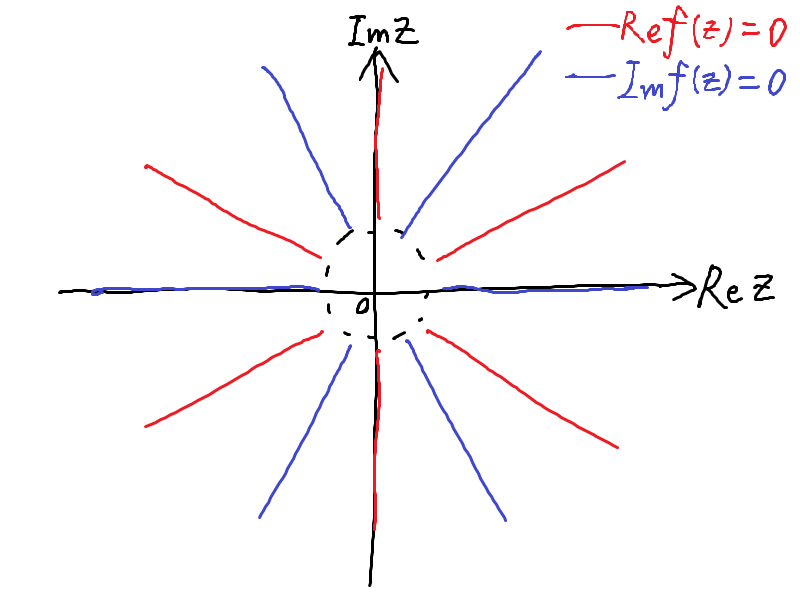
\includegraphics[width=0.33\linewidth]{fig/poly-root-outer.png}
\caption{$n=3$,$|z|$很大时$\opRe f(z)=0$和$\opIm f(z)=0$的图像}
\label{fig-poly-root-outer}
\end{figure}

其中红线为$\opRe f(z)=0$的图像,蓝线为$\opIm f(z)=0$的图像,黑圈里的情况现在还不知道,一种可能的情况如图\ref{fig-poly-root-inner},红线和蓝线的交点就是$f(z)=0$的根。
\begin{figure}[htb]
\centering
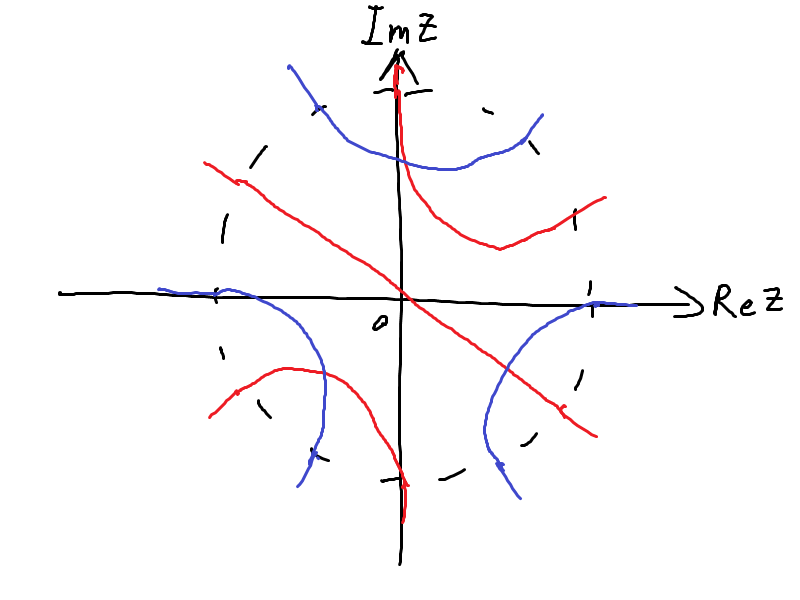
\includegraphics[width=0.33\linewidth]{fig/poly-root-inner.png}
\caption{$n=3$,$|z|$不太大时$\opRe f(z)=0$和$\opIm f(z)=0$可能的图像}
\label{fig-poly-root-inner}
\end{figure}

但是$f(z)$是一个光滑的函数,那么圈里的红线应该把圈外的红线两个一组相连,而且不会出现三条线交叉在同一点的情况,否则就不光滑了。如果四条线交叉在同一点,我们可以把交叉点分开,当作它们没有相交。蓝线也是这样。

于是“$n$次多项式有$n$个根”这个问题被我们转化为了一道炫酷的奥数题:圆周上相间排列着$2n$个红点和$2n$个蓝点,用不相交的红线把红点两个一组相连,不相交的蓝线把蓝点两个一组相连,求证红线和蓝线一定相交。用奇偶性很容易证明。

当然没有哪本高数书会讲这么炫酷的方法,我参考的是克莱因的《高观点下的初等数学》。
